\chapter{Case Study: Ovarian Cancer Survival Data}

We have data from a 1979 study that compares the effect of two different treatments for ovarian cancer\footnote{Edmunson, J.H., Fleming, T.R., Decker, D.G., Malkasian, G.D., Jefferies, J.A., Webb, M.J., and Kvols, L.K., Different Chemotherapeutic Sensitivities and Host Factors Affecting Prognosis in Advanced Ovarian Carcinoma vs. Minimal Residual Disease. Cancer Treatment Reports, 63:241-47, 1979.}. This dataset is in the \texttt{survival} R package under the heading \texttt{ovarian}. 

\section{Dataset}

The dataset contains information on the following variables for $n=26$ women:

\begin{itemize}
\item \emph{futime}: The number of days from enrollment until death or censoring, whichever came first.
\item \emph{fustat}: An indicator of death (1) or censoring (0).
\item \emph{age}: Patient's age in years at time of treatment initiation. 
\item \emph{resid.ds}: An indicator of the extent of residual disease.
\item \emph{rx}: Treatment group (1 = cyclophosphamide, 2 = cyclophosphamide plus adriamycin)
\item \emph{ecog.ps}: A measure of performance score or functional status, using the Eastern Cooperative Oncology Group (ECOG)'s scale. It ranges from 0 (fully functional) to 4 (completely disabled). Level 4 subjects are generally considered to be too ill to enter a randomized trial such as this.
\end{itemize}

\begin{center}
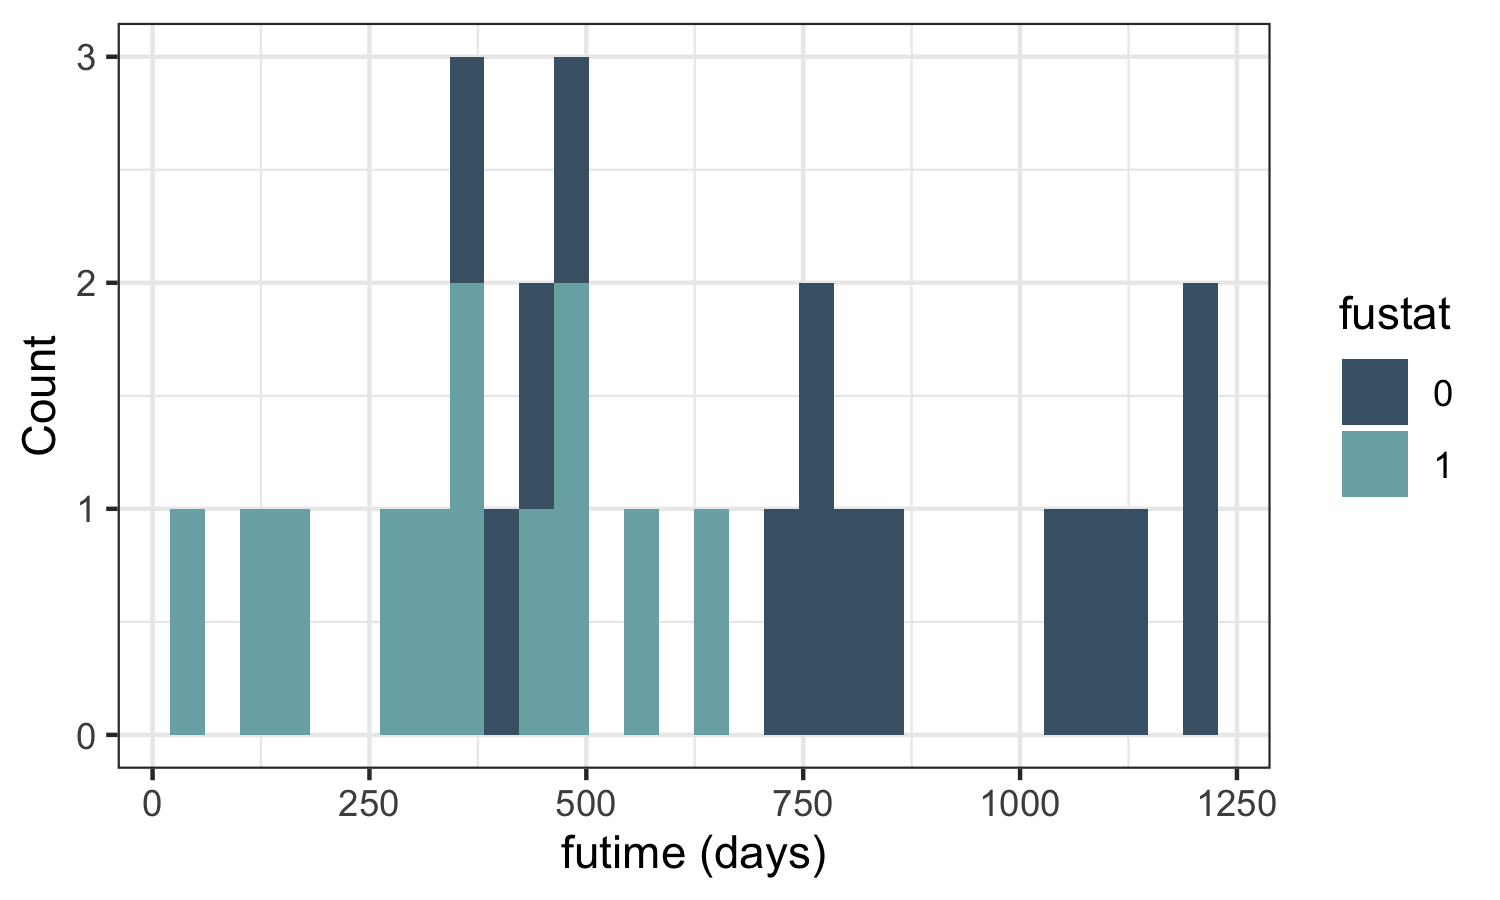
\includegraphics[width=0.3\textwidth]{img/cs-ovarian-futime.png}
\end{center}

\section{Questions}

\section{Analysis}



